\subsubsection{Risultati sperimentali}
Con l'obiettivo di migliorare le performance del sistema in modo che possa supportare il nuovo carico pesante abbiamo innanzitutto individuato il collo di bottiglia nel server B. Questo risultato era già evidente dai grafici dei precedenti obiettivi, confermato dal fatto che il bound per il throughput è:
$$\frac{1}{D_{max}}$$ $$\text{dove}\ D_{max}\ =\ \text{domanda massima}$$
Per il server B è 1.25$job/s$ quindi non può soddisfare il carico di 1.4$job/s$ richiesto. Inoltre dal seguente grafico in \autoref{fig:obj3_lineplot_throughput_comparison} si nota come i throughput più bassi siano del server B e P. Siccome non si può agire sul server P in quanto servizio esterno al sistema andiamo ad operare sul server B. 

Il miglioramento al sistema consiste nella sostituzione del server B con uno più performante. A tale scopo abbiamo selezionato tempi di servizio a partire da 0.8$s$ (attuale tempo di servizio) decrementando di 0.05$s$ fino ad arrivare a 0.4$s$ ed effettuando per ogni valore una run per ogni tasso di arrivo. Per ogni run abbiamo messo a confronto utilizzazione in \autoref{fig:obj4_utilization_service-time} e throughput in \autoref{fig:obj4_throughput_service-time}.
\begin{figure*}
    \centering
    \begin{subfigure}{1\linewidth}
        \centering
        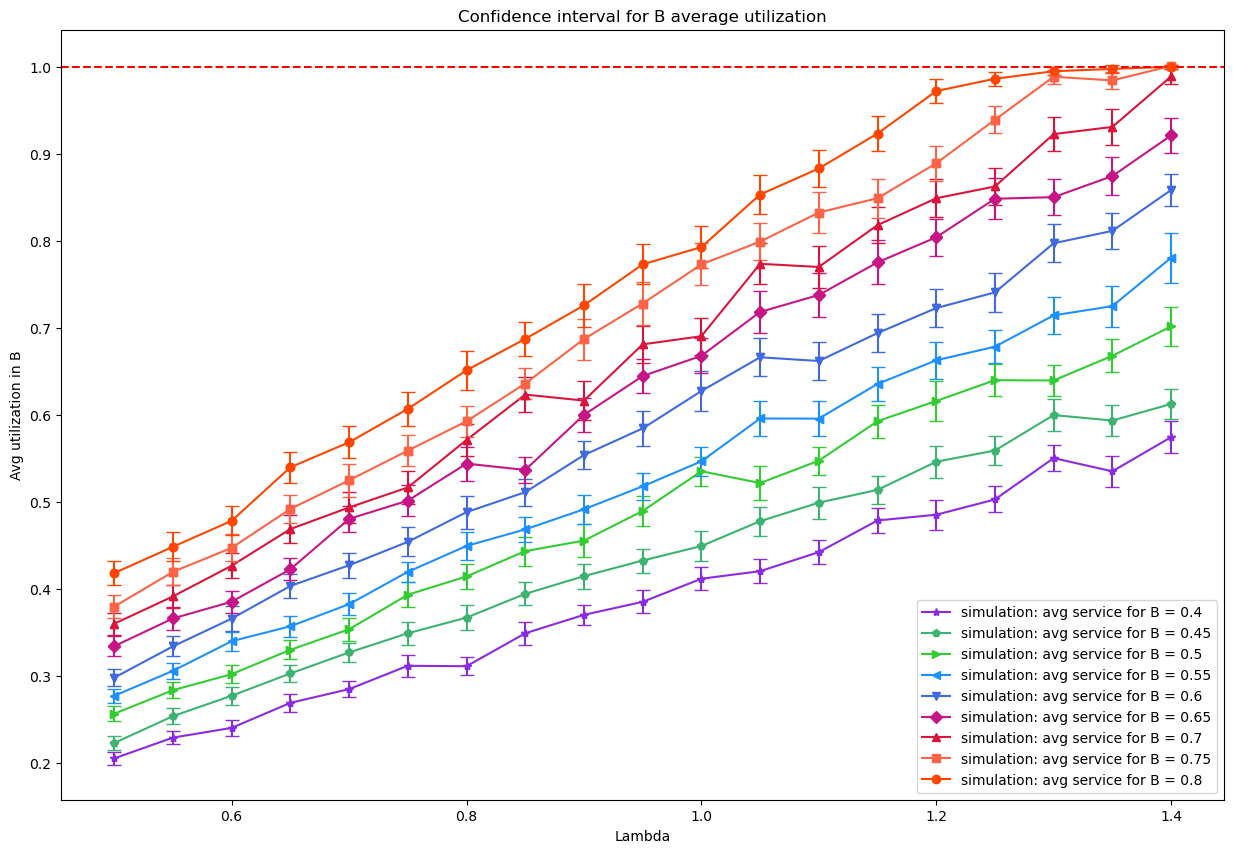
\includegraphics[width=0.8\columnwidth]{figs/results/obj4/obj4-utilization-service-time.png}
        \caption{Utilizzazione}
        \label{fig:obj4_utilization_service-time}
    \end{subfigure}
    \hfill
    \begin{subfigure}{1\linewidth}
        \centering
        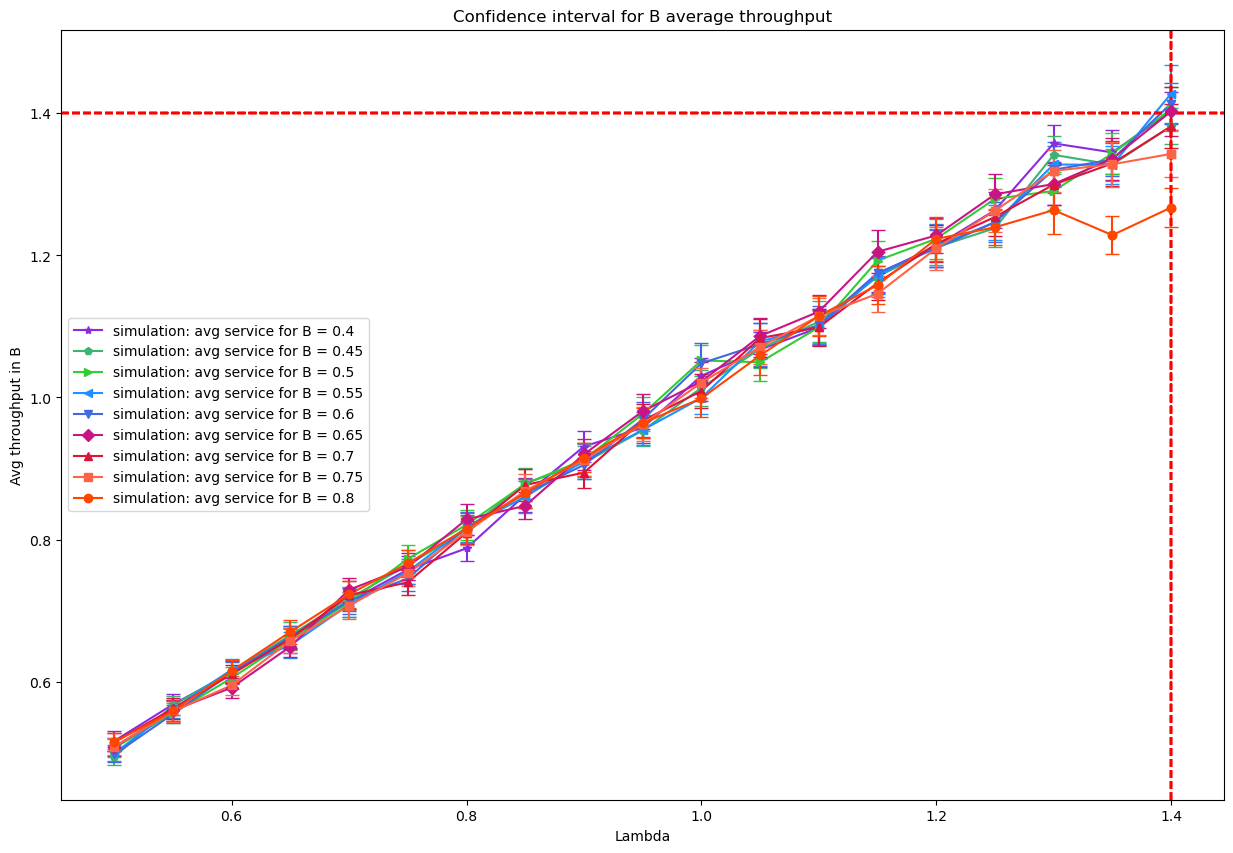
\includegraphics[width=0.8\columnwidth]{figs/results/obj4/obj4-throughput-service-time.png}
        \caption{Throughput}
        \label{fig:obj4_throughput_service-time}
    \end{subfigure}
    \caption{Confronto Throughput e Utilizzazione medi al variare dei valori dei tempi di servizio}
    \label{fig:obj4-service-time-comparison}
\end{figure*}

Dai grafici si nota come l'utilizzazione decresca notevolmente al aumentare del rate di servizio, mentre per i throughput la differenza è meno netta.\\
Abbiamo così deciso di riportare i risultati di due modelli diversi. Il primo è il più efficiente ovvero con tempi di servizio medi di 0.4$s$ ed è la stessa soluzione adottata dal caso di studio di riferimento che per throughput e utilizzazione riporta i seguenti valori minimi e massimi come si può vedere in \autoref{tab:04_metrics}:
\begin{table}
    \centering
    \caption{Minimi e massimi di utilizzazione e throughput per tempi di servizio 0.4 del server B}
    \begin{tabular}{ccc}
         $\lambda$ & metrica & valore\\
        0.5 & utilizzazione & 0.20484\\
        1.4 & utilizzazione & 0.574275\\
        0.5 & throughput & 0.516347\\
        1.4 & throughput & 1.40302
    \end{tabular}
    \label{tab:04_metrics}
\end{table}
 Per quanto riguarda il secondo modello abbiamo valutato che la spesa da sostenere per comprare un server in grado di dimezzare i tempi di servizio
può essere notevole, quando potrebbe bastare un altro server anche di poco più performante. In tale ottica abbiamo scelto il modello con tempi di servizio 0.65$s$ ottenendo un throughput massimo è di 1.4$job/s$. Abbiamo ottenuto i risultati minimi e massimi riportati in \autoref{tab:065_metrics}:
\begin{table}
    \centering
    \caption{Minimi e massimi di utilizzazione e throughput per tempi di servizio 0.65 del server B}
    \begin{tabular}{ccc}
         $\lambda$ & metrica & valore\\
        0.5 & utilizzazione & 0.333898\\
        1.4 & utilizzazione & 0.921304\\
        0.5 & throughput & 0.507752\\
        1.4 & throughput & 1.40273
    \end{tabular}
    \label{tab:065_metrics}
\end{table}
Mentre per l'utilizzazione le prestazioni degradano notevolmente, il throughput varia molto poco, possiamo quindi considerarla comunque una valida miglioria. Rappresenta inoltre, tra quelle considerate, la prima configurazione che soddisfi i requisiti, infatti già per tempi di servizio di 0.70$s$ il throughput massimo è 1.38$job/s$ e l'utilizzazione 0.98.
\subsubsection{Verifica con il modello analitico}
Per la verifica abbiamo scelto comunque il modello con tempo di servizio medi 0.4$s$. Riportiamo i grafici che confrontano l'andamento con il modello analitico per il throughput in \autoref{fig:obj4_line-throughput} e l'utilizzazione in \autoref{fig:obj4_lineplots_utilization}. Notiamo come la differenza tra i due modelli sia poca, risultato che verifica la correttezza del modello.
\begin{figure*}
    \centering
    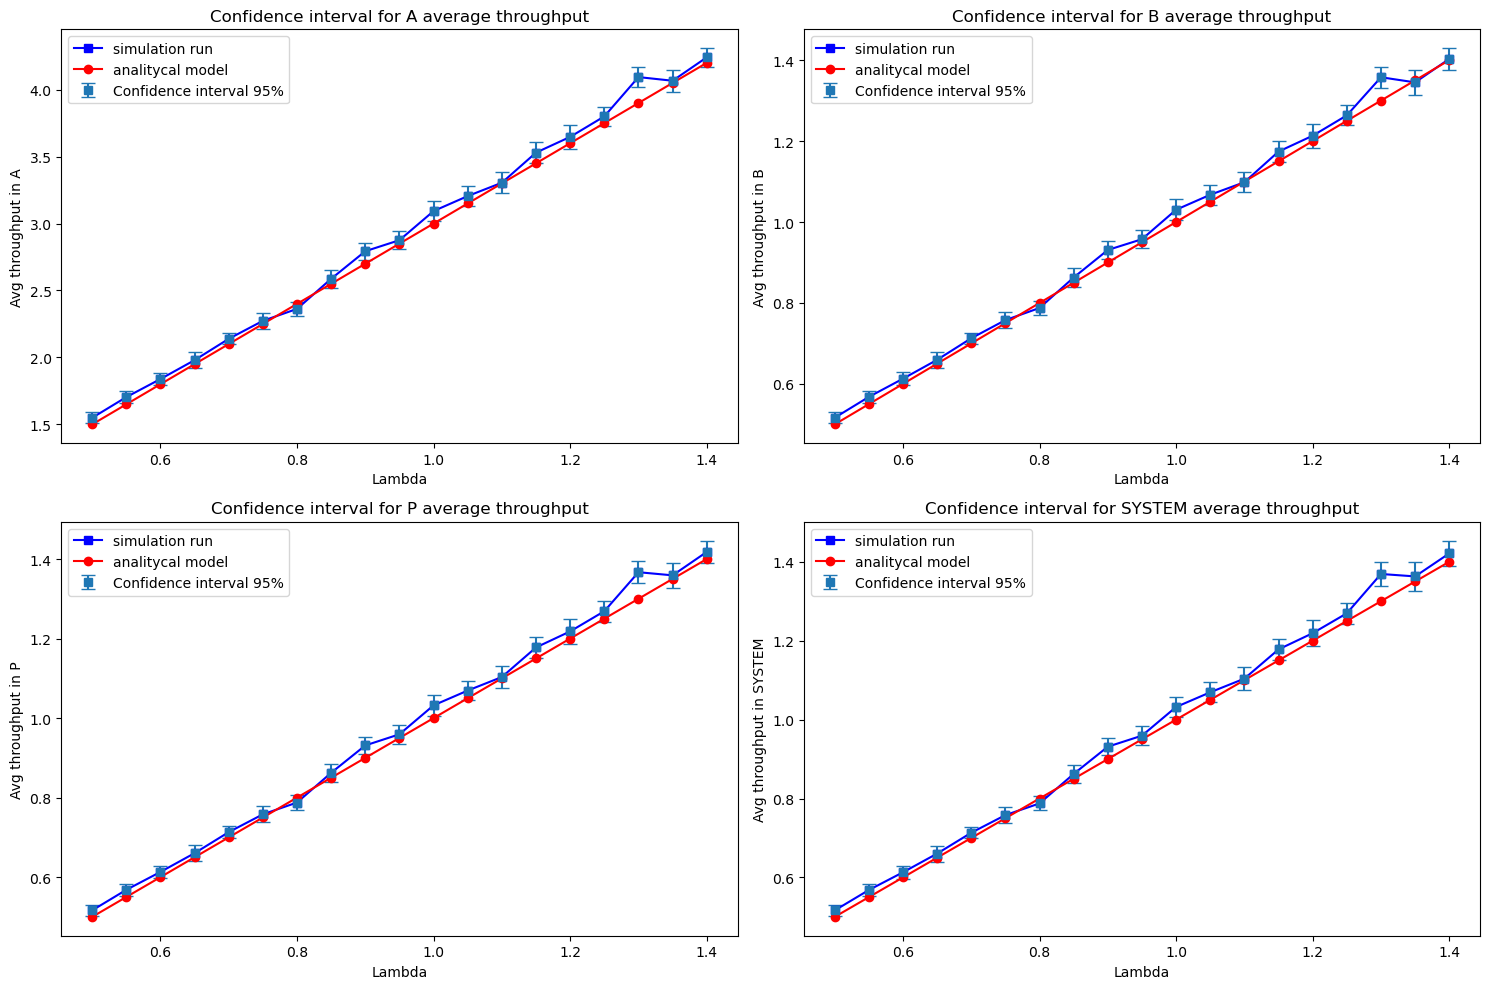
\includegraphics[width=\linewidth]{figs/results/obj4/obj4-line-throughput.png}
    \caption{Intervallo di confidenza del throughput e confronto con modello analitico per l'obiettivo 4.}
    \label{fig:obj4_line-throughput}
\end{figure*}
\begin{figure*}
    \centering
    \begin{subfigure}{0.49\linewidth}
        \centering
        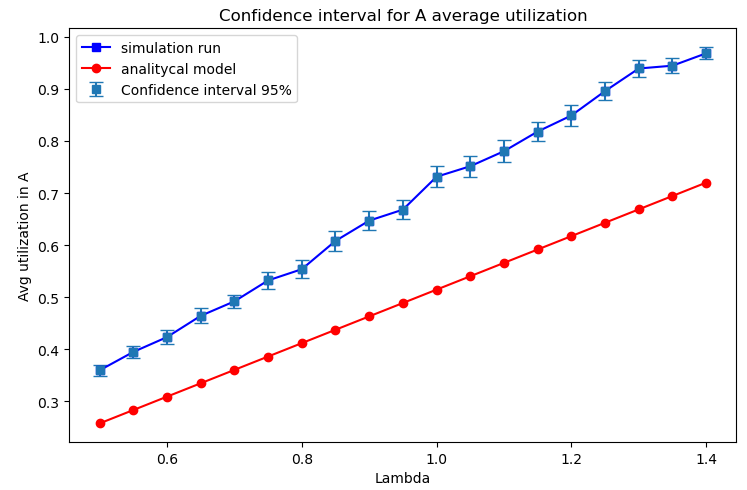
\includegraphics[width=\columnwidth]{figs/results/obj4/obj4-utilizzazione-A.png}
        \caption{Server A}
        \label{fig:obj4_line_utilization_A}
    \end{subfigure} 
    \begin{subfigure}{0.49\linewidth}
        \centering
         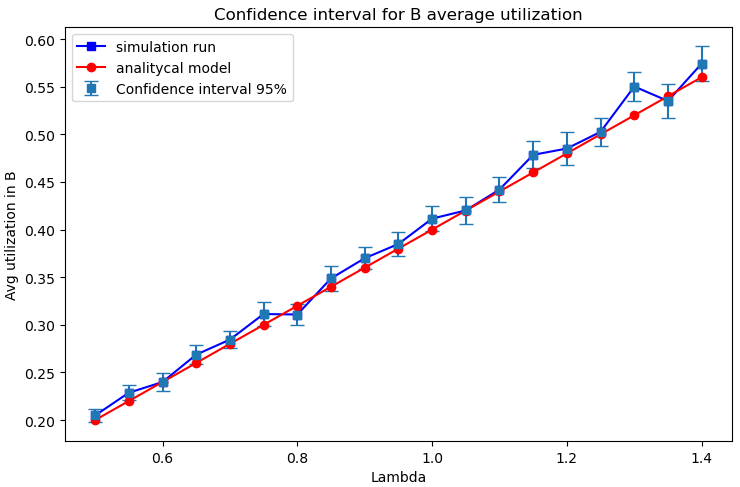
\includegraphics[width=\columnwidth]{figs/results/obj4/obj4-utilizzazione-B.png}
        \caption{Server B}
        \label{fig:obj4_line_utilization_B}
    \end{subfigure}
    \begin{subfigure}{0.5\linewidth}
        \centering
        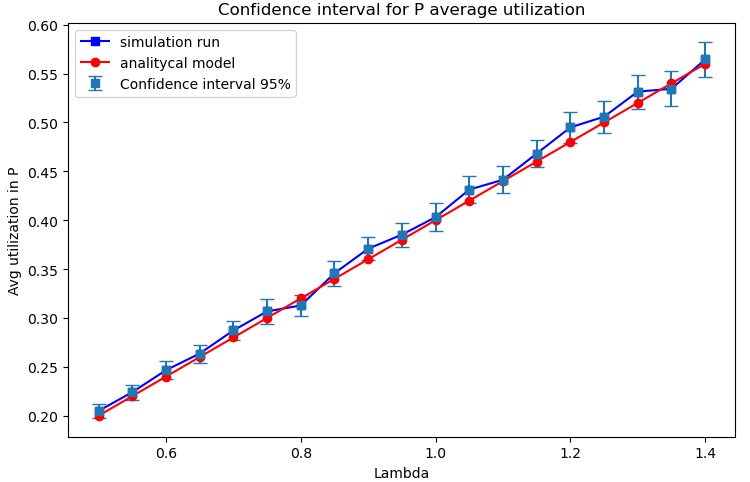
\includegraphics[width=\columnwidth]{figs/results/obj4/obj4-utilizzazione-P.png}
        \caption{Server P}
        \label{fig:obj4_line_utilization_P}
    \end{subfigure}
    \caption{Intervallo di confidenza dell'utilizzazione e confronto con modello analitico per l'obiettivo 4.}
    \label{fig:obj4_lineplots_utilization}
\end{figure*}

\subsubsection{Validazione con il caso di studio}
\label{sec:results-obj4-validation}
Per la validazione facciamo riferimento al modello con tempo medio di servizio 0.4$s$ in quanto è l'unico con cui possiamo effettuare un confronto con i risultati riportati dal caso di studio. Seguono i grafici dove vengono messe a confronto le due configurazioni, quella originale e quella migliorata nel nostro modello di simulazione \autoref{fig:obj4_validazione_simulation} e nel caso di studio \autoref{fig:obj4_validazione_casestudy}
\begin{figure*}
    \centering
    \begin{subfigure}[b]{0.49\linewidth}
        \centering
        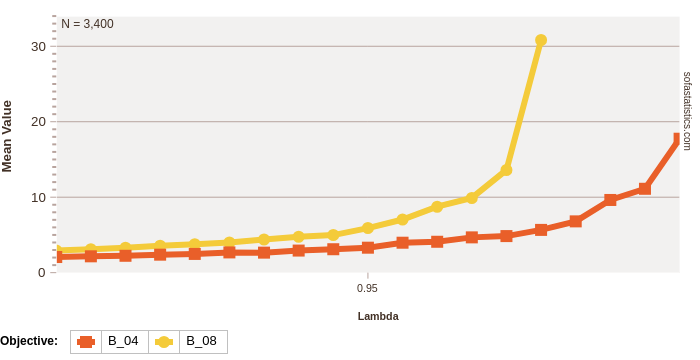
\includegraphics[width=\columnwidth]{figs/results/obj4/obj4-simulazione-validazione.png}
        \caption{Risultati sperimentali}
        \label{fig:obj4_validazione_simulation}
    \end{subfigure}
    \hfill
    \begin{subfigure}[b]{0.49\linewidth}
        \centering
        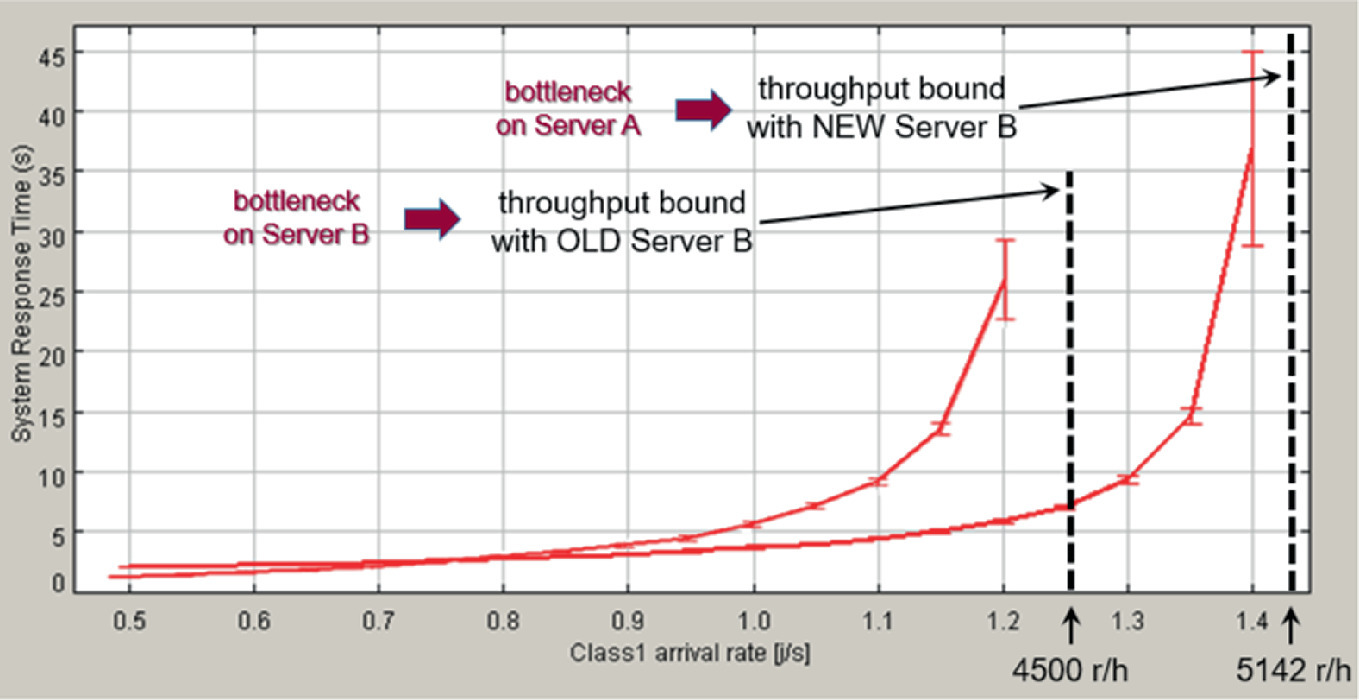
\includegraphics[width=\columnwidth]{figs/results/obj4/obj4-validazione.jpg}
        \caption{Caso di studio \citep{DBLP:books/sp/Serazzi24}}
        \label{fig:obj4_validazione_casestudy}
    \end{subfigure}
    \caption{Tempo di risposta medio prima e dopo la miglioria del server B in funzione del rate medio degli arrivi esterni}
    \label{fig:obj4_validazione}
\end{figure*}
